\documentclass[]{article}
\usepackage[utf8x]{inputenc}
\usepackage[russian]{babel}
\usepackage{hyperref}
\usepackage{amsmath}
\usepackage{amssymb}
\usepackage{cancel}
\usepackage{graphicx}
\graphicspath{ {./pictures/} }
\title{Численные методы}
\author{Александр Голованов}

\begin{document}
\maketitle
\newpage
\tableofcontents
\newpage

\section{18 февраля 2025}
\subsection{Графическое решение нелинейных систем}

\begin{gather*}
\begin{cases}
3x-y =-10\\
x^2+y=10
\end{cases}
\end{gather*}

\begin{figure}[h]
\caption{Графики}
\centering
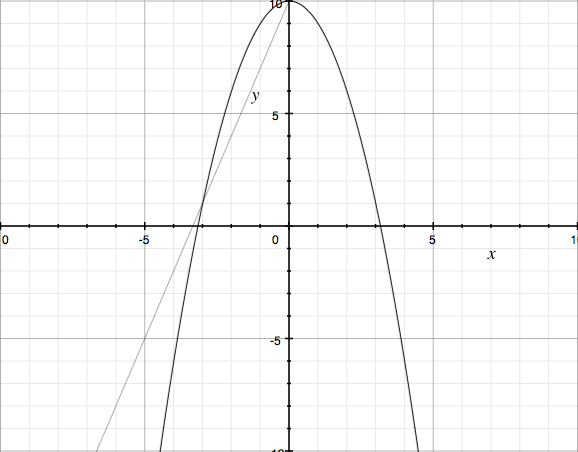
\includegraphics[width=\textwidth]{graph1}
\end{figure}


\end{document}